\section{Desarrollo}

\subsection{Ejercicio 1}
TODO: AGREGAR ALGO

\subsection{Ejercicio 2}
TODO: AGREGAR ALGO

\subsection{Ejercicio 3}
TODO: AGREGAR ALGO

\subsection{Ejercicio 4}
TODO: AGREGAR ALGO

\subsection{Ejercicio 5}
TODO: AGREGAR ALGO

\subsection{Ejercicio 6}
TODO: AGREGAR ALGO

\subsection{Ejercicio 7}
TODO: AGREGAR ALGO

\subsection{Ejercicio 8}
TODO: AGREGAR ALGO

\subsection{Ejercicio 9}

Para mostrar con un ejemplo un caso que no sea factible para el scheduler RM y si lo sea para EDF nos basto el siguiente lote de 2 tareas periodicas:

Nota: Para simplicar el ejemplo consideramos en este caso despreciable el tiempo de cambio de contexto.
\\
\\
Lote:
\verbatiminput{graficos/lotes_ej9.tsk}

Produciendo los siguientes gráfico:

Para RM:

\begin{center}
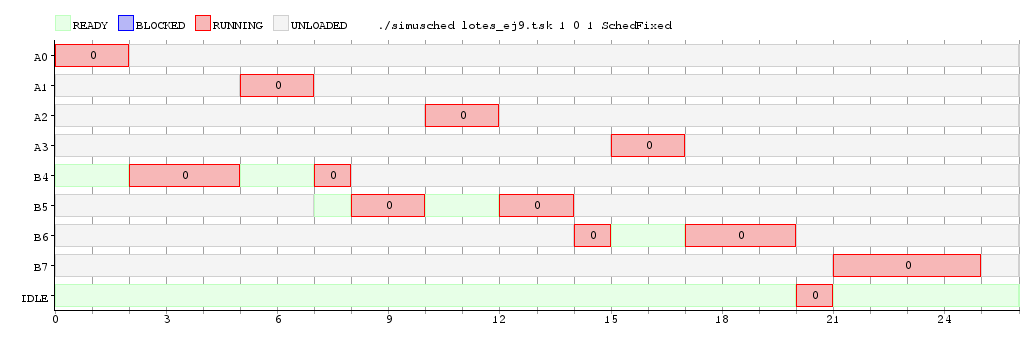
\includegraphics[scale=0.4]{graficos/eje9_fixed.png}
\end{center}

Para EDF:

\begin{center}
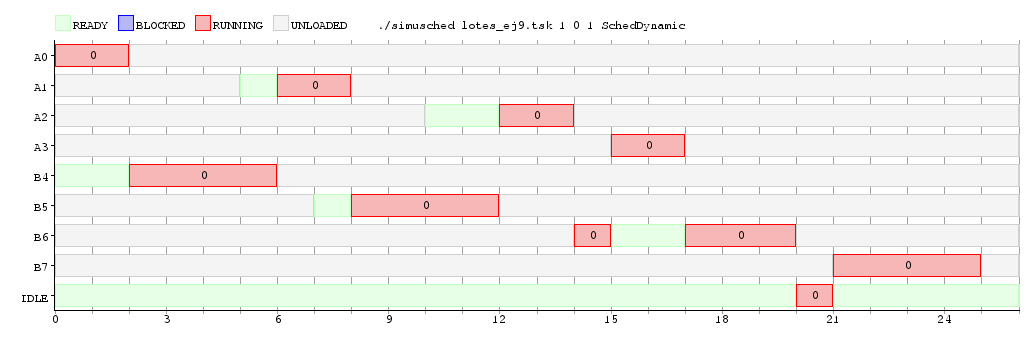
\includegraphics[scale=0.4]{graficos/eje9_dynamic.png}
\end{center}

La tarea de la familia A tiene un periodo menor que el de la familia B por lo cual según el scheduler RM tiene mayor prioridad asignada. Esta elección de priorizar a la familia A provoca un perjuicio en la familia B por lo que la familia B no puede cumplir su deadline en $T=7$ (Se produce un overflow).

En el caso del gráfico de EDF se puede observar que le da el CPU un poco más a la familia B por tener el deadline más próximo logrando evitar así el inclumplimiento del deadline (en $T=5$ deja esperando a la tarea de la familia A).

Algo interesante para destacar es que en este caso ambos scheduler ocuparon el mismo tiempo el CPU con trabajos, lo que cambia es que el scheduler RM a diferencia de EDF tiende a gastar más tiempo de computo en tareas de mayor prioridad dejandolo poco procesamiento a las de menor prioridad.

\subsection{Ejercicio 10}
//TODO: AGREGAR TEXTO

\begin{center}
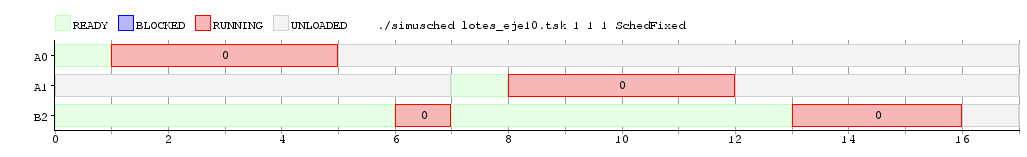
\includegraphics[scale=0.4]{graficos/eje10_Fixed.png}
\end{center}

//TODO: AGREGAR TEXTO
\begin{center}
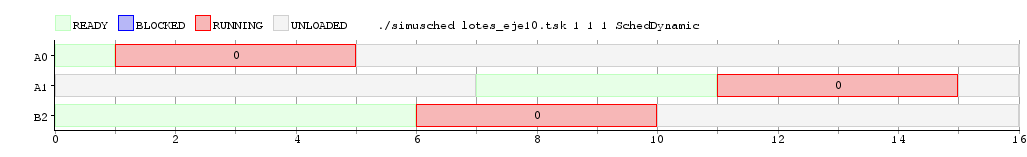
\includegraphics[scale=0.4]{graficos/eje10_Dynamic.png}
\end{center}
